\chapter{Introduction}

\section{Objectif du projet}

Le but de ce projet est de découvrir une nouvelle technologie concernant l'automatisation, le
déploiment, le clustering ou encore le cloud. Cela nous permettra de découvrir différents outils
que l'on sera peut-être amené à manipuler dans le futur.

\section{Présentation de la technologie}

\subsection{Docker}

\columnratio{0.6}
\begin{paracol}{2}

Docker est une plateforme open-source permettant de concevoir, tester et déployer rapidement des
applications. Il utilise la notion de conteneurs qui, comme la virtualisation, permet d’isoler
une application de la machine hôte tout en étant plus léger et plus simple à déployer.

\switchcolumn


\includegraphics[width=0.7\linewidth]{img/docker}

\end{paracol}
\jmp

Docker étend les conteneurs LXC qui s’appuient sur les fonctionnalités du noyau pour l’isolation
(namespaces, cgroups), en fournissant une API haut niveau, plus simple d’utilisation.\newline

Comme on peut le voir sur la figure \ref{fig:diffvm}, la différence principale entre un conteneur 
et une machine virtualisé est que dans le premier cas le système d'exploitation n'est pas émulé.
Le conteneur utilise le noyau de la machîne hôte, et utilise les mécanismes de namespaces et de 
CGroups (entre autres) afin de s'isoler de la machine hôte.

\begin{figure}
    \centering
    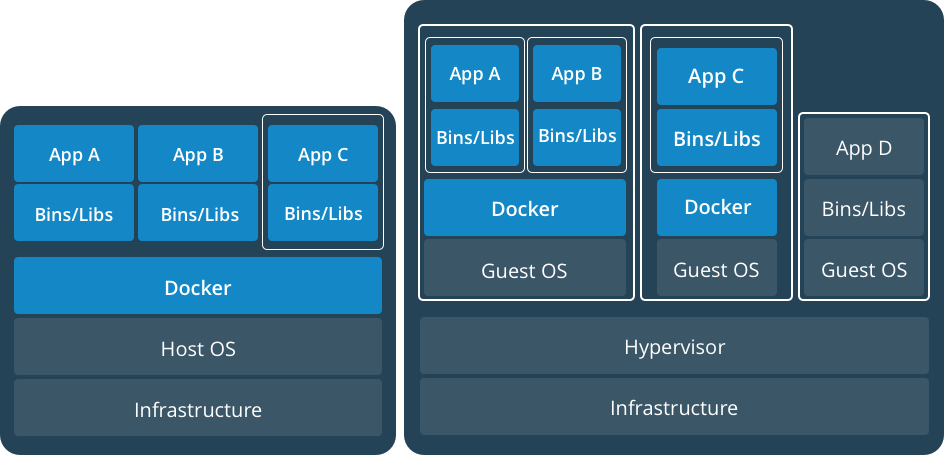
\includegraphics[width=\textwidth]{img/vm-container}
    \caption{Différences entre virtualisation et conteneurs}
    \label{fig:diffvm}
\end{figure}

Cela donne l'avantage aux conteneurs d'être plus rapide et léger car stocker et émuler un noyau
et un système d'exploitation demande plus d'espace disque, de mémoire vive et de puissance de
calcul. Enfin cette légereté font que les conteneurs sont plus facilement déployable.

Cependant à la différence d'une machine virtuelle, ce n'est pas une isolation complète, et donc
si l'application est critique est nécessite un fort niveau d'isolation, mieux vaut utiliser une
machine virtuelle.\newline

Il existe également une bibliothèque d’images publics, le Docker Hub, permettant de créer
facilement tous types de conteneurs.

\subsection{Swarm}

\begin{figure}[h!]
    \centering
    
\includegraphics[width=0.5\textwidth]{img/swarm}
    \caption{Logo de Swarm}
\end{figure}

\chapter{Interêts}

\section{Interêt du clustering}

\section{Pourquoi utiliser Docker Swarm ?}

\chapter{Installation}

\chapter{Utilisation}

Un \verb:swarm: consiste en plusieurs nœuds docker qui
s'exécute en mode swarm. Les nœuds docker peuvent avoir deux types: 
\begin{itemize}
    \item Un manager (\verb:manager:) s'occupe de la gestion de permissions et de l'attribution 
        des tâches.
    \item Un travailleur (\verb:worker:) effectue les tâches que lui attribue le manager.
\end{itemize}

Il est possible pour un même nœuds d'endosser deux rôles simultanèment.

\section{Commandes de bases}

Les commandes du mode \verb:swarm: de docker sont les suivantes:
\begin{itemize}
	\item \verb:swarm init:: Initialise un \verb:swarm:. Le nœuds docker ciblé par 
        cette commande devient un manager pour un nouveau \verb:swarm: initialement vide.
	\item \verb:swarm join:: Permet à un nœuds docker de rejoindre un \verb:swarm: existant
        en indiquant le token fournis par la commande \verb:swarm init:.
    \item \verb:swarm leave:: Permet à un nœud de quitter le \verb:swarm:, pour retirer un 
        manager de l'essain il faut utiliser l'option \verb:--force:.
\end{itemize}

\section{Un cas d'utilisation}

On va maintenant mettre en place un \verb:swarm: avec un manager et deux workers. Afin de
simuler un réseau de plusieurs machines on va installer \verb:docker: sur des conteneurs
lxc en utilisant le script d'installation fournis en annexe. Le montage réseau est le suivant:
\begin{bash}
NAME           STATE            IPV4        
docker-manager RUNNING 10.0.3.111, 172.17.0.1
docker-worker1 RUNNING 10.0.3.235, 172.17.0.1
docker-worker2 RUNNING 10.0.3.203, 172.17.0.1
\end{bash} 
\begin{center}
    \emph{les adresses \verb:172.17.0.1: correspondent à l'interface docker0}
\end{center}

\newpage
On commence donc par créer un \verb:swarm: depuis le conteneur du manager:
\begin{bash}
docker swarm init
Swarm initialized: current node (qt9wx5u1hegtv8mjg61zbxnob) is now a manager.
To add a worker to this swarm, run the following command:
    docker swarm join --token SWMTKN-1-5oug0mpki7... 10.0.3.111:2377
\end{bash}
On note le token afin de pouvoir l'utiliser plus tard. On peut vérifier le status de 
ce nœud avec la commande \verb:docker node ls: qui produit la sortie suivante:
\begin{bash}
ID                        HOSTNAME         STATUS    AVAILABILITY   MANAGER
qt9wx5u1hegtv8mjg61zbxnob docker-manager   Ready     Active         Leader
\end{bash}
Ce qui confirme bien que l'essaim à été créé. On va maintenant ajouter les deux worker à notre 
essaim, on se connecte sur chacun des conteneurs et on utilise la commande suivante:
\begin{bash}
docker swarm join --token SWMTKN-1-5oug0mpki7... 10.0.3.111:2377
This node joined a swarm as a worker.
\end{bash}
Si on se reconnecte sur le conteneur du manager et que l'on lance à nouveau la commande
\verb:docker node ls:, on peut voir que l'essaim comporte bien 3 machines:
\begin{bash}
ID                          HOSTNAME         STATUS    AVAILABILITY   MANAGER
qt9wx5u1hegtv8mjg61zbxnob * docker-manager   Ready     Active         Leader 
u2g1r24whkfz34mwn8rb9ovrs   docker-worker1   Ready     Active                
73t7ozstyb7d312888879i6um   docker-worker2   Ready     Active                
\end{bash}
On doit à présent déployer un service sur notre essaim. On va utiliser dans pour cette exemple
le cas d'un service web dont on souhaite répartir la charge sur les 3 conteneurs. On va pour cela
utiliser le serveur web \verb:nginx:. On lance la commande suivante depuis le manager 
pour créer un service web répartis entre les conteneurs:
\begin{bash}
docker service create --name my_web --replicas 3 --publish 8080:80 nginx
\end{bash}
\begin{itemize}
    \item \verb:--name:: permet d'indiquer le nom de ce service.
    \item \verb:--replicas:: indique le nombre de nœuds de l'essaim auquel on souhaite
        attribuer cette tâche, ici 3.
    \item \verb:--publish:: permet d'indiquer que l'on souhaite rediriger tous le traffic 
        entrant sur le port 8080 du conteneur lxc sur le port 80 du service docker.  
\end{itemize}
Il est important de noter que l'option \verb:--publish: en plus de faire la redirection,
active le mode \verb:routing mesh:. Ce mode permet de faire de l'équilibrage de charge de
manière transparente pour le client, en effet une requête effectué sur un nœud de l'essaim 
peut être traité par un autre nœud si le premier nœud est indisponible. 

\newpage

Pour l'instant on peut vérifier que le service \verb:my_web: fonctionne sur l'ensemble des
nœuds de l'essaim, pour cela on utilise la commande suivante:
\begin{bash}
docker service ps my_web
ID           NAME     IMAGE        NODE           DESIRED STATE
8z15jsh81yzb my_web.1 nginx:latest docker-manager Running      
wbh4bodsezqa my_web.2 nginx:latest docker-worker1 Running      
ou5pyyrpr6k1 my_web.3 nginx:latest docker-worker2 Running       
\end{bash}
Il est possible de se connecter sur l'une des interfaces web en allant par exemple sur 
\url{http://10.0.3.111:8080/}
\begin{figure}[h!]
    \centering
    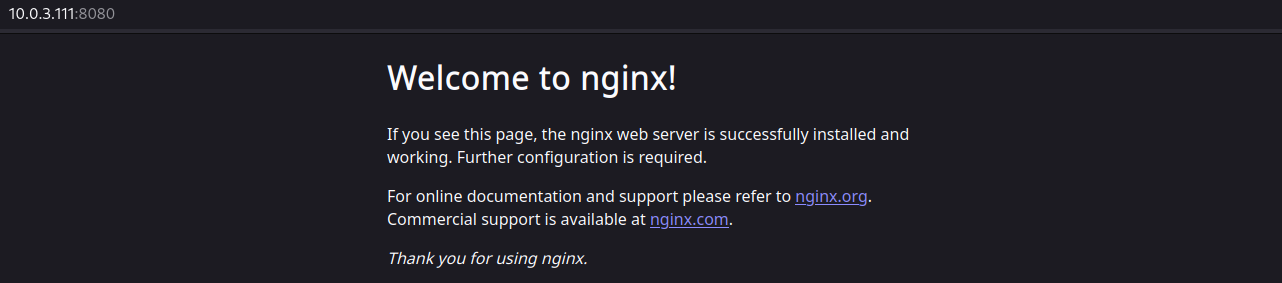
\includegraphics[width=15cm]{img/nginx}
    \caption{Page par défault de nginx}
\end{figure}

\chapter{Configuration}

\section{Performances}

\section{Sécurité}

\section{Disponibilité}
Si on arrête le conteneur lxc \verb:docker-worker1:, puis que l'on se connecte sur le
conteneur du manager afin d'afficher l'état de l'essaim on obtient ceci:
\begin{bash}
docker service ps my_web
ID           NAME         IMAGE        NODE           DESIRED STATE   
8z15jsh81yzb my_web.1     nginx:latest docker-manager Running         
41hbyfhleu1l my_web.2     nginx:latest docker-worker2 Running        
wbh4bodsezqa  \_ my_web.2 nginx:latest docker-worker1 Shutdown      
ou5pyyrpr6k1 my_web.3     nginx:latest docker-worker2 Running      
\end{bash}
On peut voir que le conteneur docker-worker2 à récupèrer la tâche du worker1 de manière
autonome et transparente, ce qui veut dire qu'en cas de panne ou autre indisponibilité, 
docker équilibre automatiquement la charge.


\chapter{Conclusion}
